In this chapter we will describe the application overview. Next the extension of KEMS will be explained and its API will be introduced. Later we will talk about the library ASP.NET API 1.0 which was utilised in our CAPI and how we managed ATs. Lastly the KenticoApp will be detailed. The languages CSS, HTML and JS leveraged with JQM will be described along with the usage og AJAX.
\section{Application Overview}
\begin{figure}[ht!]
  \centering
  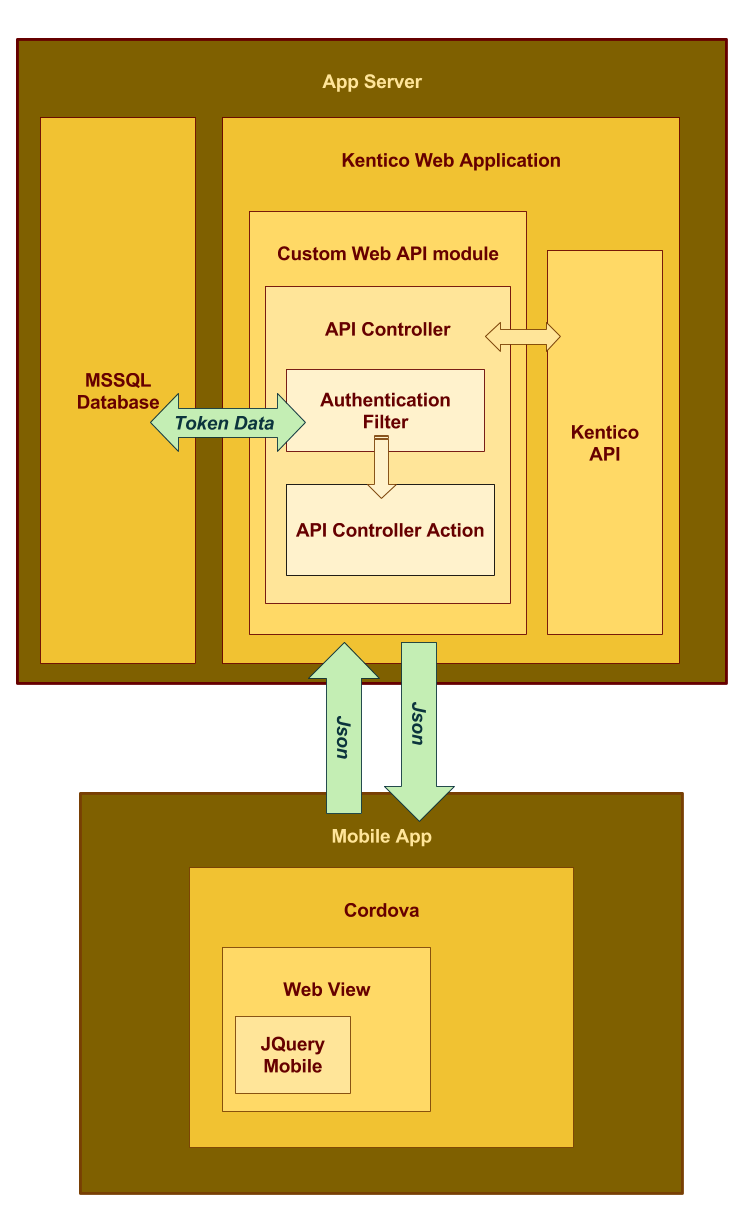
\includegraphics[width=0.8\textwidth]{Images/Architecture.png}
  \caption{Architecture overview}
  \label{architectureOverview}
\end{figure}
This thesis consists of two parts. The first of which is the~CAPI back-end. It stores and retrieves data from and to the database via calls to the KAPI. It itself is called by the second part - the~mobile client app, called KenticoApp, through which the~user is able to communicate with the~system and manage his site. The visual representation of the architecture is demonstrated in the figure \ref{architectureOverview}. The image shows the app server and the mobile app communication via JSON and how the components are nested. Our CAPI is nested in the Kentico web app which is hosted on the app server. The controllers are nested in the CAPI and are communicating with the Microsoft structured query language (MSSQL) database through the Authentication Filter which checks whether an API action will be executed. The KAPI communicates with the controllers. The KenticoApp is the mobile app which utilises the ACF and its web view with JQM. 

The CAPI partially follows the REST architecture by using appropriate HTTP methods. For example we use POST requests for creating or GET requests for reading resources from the back-end. The usage of status codes, such as 200, 403 or 503 is also a RESTful convention. Our back-end is stateless. This is achieved by using ATs instead of storing the user session across multiple HTTP requests. One of the reasons why we cannot call this application RESTful is it does not follow the fundamental concept of identifying all resources and relationships between them. For example our \textit{System} "resource" contains the method \textit{ClearCache()} and \textit{ShowEventlog()}. These should be identified in separate resources \textit{CacheClearer} and \textit{Eventlog}. Further description of the CAPI can be found below.

The KenticoApp is a mobile app which can be used by global admins. It offers a welcome page where the user has to sign in. If the authentication is successful and the user has the proper authorization, the user is redirected to a menu page with three buttons and their descriptions, each one representing a controller in the CAPI. From there on the user can choose what action to conduct. A layout with options such as view the current user or logout is available. It also contains the breadcrumbs to the current page. 

The communication between the CAPI and KenticoApp is ensured by AJAX using JSON format. It is an effective way to broadcast information via a simple string.

\section{Extending Kentico} \label{implExtendingKentico}
To be able to add functionality to KEMS a new project we called CAPI had to be created in the already existing solution which was installed with the installation of KEMS. The  project then was registered using a Kentico module ASP.NET API 1.0. This will be described in the subsections \ref{cutomModule} and \ref{API1.0}
The CAPI was implemented using the .NET framework. It uses KAPI calls and is called by the KenticoApp. For executing an API call, the user has to be signed into the system and have the proper authorization. 
\subsection{Custom Kentico Module} \label{cutomModule}
The module was created as a file with the \textit{[assembly: RegisterModule(typeof(CustomWebApiModule))]} annotation and it was added into CAPI. It must inherit from the \textit{CMS.DataEngine.Module} class. We adjoined an empty constructor and overrode the \textit{CustomWebApiModule.OnInit()} method. We will discuss the content of this method later \ref{API1.0}. 
\subsection{Kentico 9.0 API}
Once the project is registered the functionality can be added. To access the features of KEMS we use KAPI. Its calls are divided into modules regarding the namespaces\footnote{A namespace represents a group of classes with related functionality}. To be able to utilise a call the respecting module has to be imported into the project as a reference first. For example in the \textit{EditUser()} method an API call which operates the \textit{UserInfo} class is used. This class is of the namespace \textit{CMS.Membership}, therefore of the same called module. We added a new reference to the module, then imported the namespace into our file with the keyword \textit{using} followed with the namespace and from there on the class could be used. This practise offers less loaded libraries which results for example into time saving when compiling the project or migrating it. 

\section{Web API Application}
As mentioned previously, to allow the user to access the KAPI from a front-end mobile app the CAPI had to be created. The proccess is described in the subsections following.
\subsection{ASP.NET API 1.0}
\label{API1.0} To allow a module to be registered to KEMS the method \textit{Configure(WebApiConfig.Register)} of the class \textit{System.Web.Http.GlobalConfiguration} must be called in the overridden \textit{CustomWebApiModuleOnInit()} method. ASP.NET API 1.0 provides several components which make it easier for us to create an API for our application, one of which is the \textit{System.Web.Http.ApiController}. All of our controllers inherit from it. One of its features is it enables the programmer to return the SC and possibly a JSON representation of the data we want to return. Another component is the \textit{System.Web.Http.Filters.ActionFilterAttribute} which is inherited by the filter in the CAPI. It allows to implement the method \textit{OnActionExecuting()}. This method is called before the execution of an API action. It is usually used when lading data from a database which are then used by big numbers of different actions. If these data are loaded into the \textit{actionContext} they can be used by all those actions and time is saved. Also the execution of an action can be prohibited. The filter we use in CAPI checks if the user attempting to carry out a task provided a valid AT. It stores the user information if the AT is valid and if it is not it prevents the task to be performed. Additional benefits of ASP.NET Web API 1.0 include making it possible to use the annotation \textit{[Route("myapi/students")]} which indicates the location no the web server from where the following method can be called. It also offers the usage of HTTP method tags such as \textit{HttpPost} or \textit{HttpGet}. These annotations specify the type of the operation, e.g. whether the server should create a new resource or just return data. Calling the action with a different method than specified is not possible. Another feature it provides is it parses a request and the programmer can then read it as a \textit{[FromBody]JObject postData} attribute. This attribute represents the JSON data sent in the body of the request from a third party application. 

Since source code on the front-end can be easily read and modified by unauthorized users, security measures should be implemented in the back-end app. To secure our system we use access tokens (ATs) and a filter. Filters are used to prevent unauthorized users from executing operations. They are noted through annotation, e.g. \textit{[Authorizator]}, either in front of a particular method, or in front of a whole controller so that all its methods are affected. The filter we use is called \textit{Authorizator} and, as already stated, it inherits from the \textit{ActionFilterAttribute}. It was implemented as our custom authorization filter and checks if the user is authenticated and if he is a global admin since only global admins are permitted to use the KenticoApp. If not, the SC 403 is returned.
CAPI uses controller classes to divide functionality into section for better overview and security. Each controller contains methods mainly affecting resources represented by it. In this thesis four controllers were implemented: \textit{AuthenticationController}, \textit{AuthorizationController}, \textit{UserController} and \textit{SystemController}. Each one of these controllers symbolizes a group of related functionality. For example the \textit{AuthorizationController} contains methods for managing roles and permissions. 
The API call structure is demonstrated in the illustrated code below. This specific call edits a user.
\lstset{style=sharpc, numbers=left}
\begin{lstlisting}
[Authorize]
[HttpPost]
[Route("kenticoapi/users/edit-user")]
public HttpResponseMessage EditUser([FromBody]JObject postData)
{
  string username, firstName, surname;
  try
  {
    username = postData["username"].ToObject<string>();
    firstName = postData["firstName"].ToObject<string>(); 
    surname = postData["surname"].ToObject<string>();
  }
  catch (Exception e)
  {
    return Request.CreateResponse(HttpStatusCode.ServiceUnavailable, new { errorMessage = e.Message });
  }
  try
  {
    UserInfo updateUser = UserInfoProvider.GetUserInfo(username);
    if (updateUser != null)
    {
      updateUser.FirstName = firstName;
      updateUser.LastName = surname;
      UserInfoProvider.SetUserInfo(updateUser);
    return Request.CreateResponse(HttpStatusCode.OK, new { user = updateUser });
    }
  } catch(Exception e)
  {
    return Request.CreateResponse(HttpStatusCode.ServiceUnavailable, new { errorMessage = e.Message });
  }
  return Request.CreateResponse(HttpStatusCode.ServiceUnavailable, new { errorMessage = "User is null" });
}
\end{lstlisting}
The annotation from the 1st line is our custom \textit{AuthenticationFilter} and checks if the user is authenticated so the call can be executed. If successfully authorized, the user is stored into the request properties from where he can be retrieved with the following command:
\lstset{style=sharpc, numbers = none}
\begin{lstlisting}
	UserInfo user = (UserInfo) Request.Properties["LoggedUserInfo"]
\end{lstlisting}
as it is done in the method \textit{GetCurrentUser()}.
Line 2 ensures that only POST requests are handled by the method. POST requests send data from the client to the server as opposed to GET requests which demand data from the server. In this example the system stores updated user information from the KenticoApp into the database. The 3rd line represents the route where the call can be accessed through the client app. The 4th line is the head of the method. Its return type enables the client to receive a \textit{StatusCode} and a value, which is the content of the HTTP response message. The parameters are passed on from the client as one object in the JSON format. On the lines 6 to 12 the JSON object is parsed into separate parameters as \textit{strings}. This is done in a \textit{try-catch} block to handle possible exceptions and return the proper response message on the line 15. The \textit{CreateResponse()} method is of the class \textit{Request} and its parameters are the status code \textit{503} and an object with the error message of the caught exception from line 13. The line 19 gets the user using the parsed \textit{username} and stores it in the variable called \textit{updateUser} of the type \textit{UserInfo}. This type is defined in the KAPI documentation and has attributes such as \textit{username}, \textit{user ID}, \textit{user first} and \textit{last name}, etc. Line 20 checks if the \textit{updateUser} is not \textit{null}. Lines 22 and 23 change the \textit{updateUser}'s first and last name. On the line 24 the \textit{updateUser} is inserted in the database. Line 25 returns the status code \textit{200} and the \textit{updateUser} object, which is later converted into JSON format. The lines 27 to 30 are similar to lines 13 to 16. If \textit{updateUser} is \textit{null} the response status code is \textit{503}, the same as on line 15, and the error message \textit{"User is null"}. 

\subsection{CAPI Token Management}
For user authentication we decided to use ATs. ATs are leveraged to secure the communication between a user and the system. After signing in the user is given a random generated unique AT by the system which stores it in its database. Before every API call, the system requires the user's AT and then checks it against the database. For the call to be executed the AT has to exist in the database with the corresponding user ID and must not be expired. If this is not the case the user is redirected to the welcome page, where he has to sign in. To represent and store the ATs in the database in our project we were inspired by the layered application design pattern, more specifically by its data access layer (DAL). This pattern is used to ensure security and scalability of an application by partitioning it into three layers. The first and lowest layer is needed to operate the database. It is called DAL and contains entities which are depictions of objects. The next layer is the business logic layer which contains the logic of the system. And the last one is the presentation layer, utilised to display the application through a UI to users. For the purpose of this thesis we decided to represent the ATs as an entity using the Entity Framework. The entity contains the user identification (ID), a unique pseudo-random code and an expiration date and time (expiration) as can be seen in the following example code. 
\lstset{style=sharpc, numbers=left}
\begin{lstlisting}
 public class Token
    {
        [Required]
        public int UserID { get; set; }
        [Required][Key]
        public string Code { get; set; }
        [Required]
        public DateTime Expiration { get; set; }
    }
\end{lstlisting}
The ID is of the type \textit{int} and is equal to the user's ID who "owns" the AT. The code is type \textit{string} and is generated with the pseudo-random number generator \textit{Random}. \textit{The chosen numbers are not completely random because a mathematical algorithm is used to select them, but they are sufficiently random for practical purposes.}\cite{msdn_documentation_system_random} Right after generating the code is tested against the database if no AT with the same one exists. If the code is already taken, another one is generated and tested. If not, the token entity is assigned the code, user ID and date and time 10 minutes from the assignment. The expiration is of the type \textit{DateTime}. After every executed API call the AT's expiration is set to 10 minutes from calling. 
Before every API call the system searches its database for expired ATs and deletes them. 

\section{Cordova Mobile Application}
To enable a user to use the CAPI a front-end mobile app had to be created. We already specified that for this purpose ACF with JQM was used.
\subsection{HTML, CSS, JS}
As mentioned earlier, due to browser differences it can be time consuming to use these languages and the soulution can be to use a framework such as JQM. It is an~open source HTML5-based UI framework and it allows users to design aesthetically pleasing mobile elements by utilising the~languages CSS and HTML. It also assigns properties to these elements. 
\lstset{style=sharpc, numbers=left}
\begin{lstlisting}
<div role="main" id="welcomePageBody" class="ui-content">
  <span data-position-to="window">
    <img src="Kentico_logo.png" id="kentico_logo" alt="kentico_logo" style="width:280px">
  </span>
  <span class="push-down">
    <label for="usrname-input">Username:</label>
    <input id="usrname-input" placeholder="Username" required />
    <label for="passwrd-input">Password:</label>
    <input id="passwrd-input" input type="password" required />
    <button id="login-btn" data-role="button" class='ui-btn ui-btn-inline ui-corner-all ui-shadow pull-right'>Log in</button>
  </span>
  <div id="error-msg" class="not-displayed"></div>
</div>
\end{lstlisting}
\begin{SCfigure}
  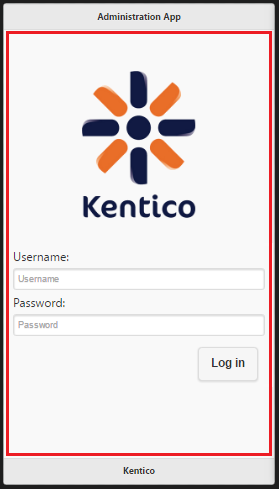
\includegraphics[width=\textwidth/2]{Images/WelcomePageIllustration.png}
  \caption{KenticoApp Welcome Page UI.}
  \label{WelcomePageIllustration}
\end{SCfigure}
The sample code above creates a tag with an image, two text fields, their labels and a button. The visualisation is shown in figure \ref{WelcomePageIllustration}. The content in the red quadrilateral in the image is the graphical representation of the code sample above. It was created as a print screen of the KenticoApp. On the first line a \textit{div} element contains a part of the page. \textit{Div} tags divide the page into smaller fractions to diverse the styles, alignments or to create groups for selection. The \textit{role="main"} attribute of the JQM library binds predefined behaviour to the content of this \textit{div}, for example it will be placed between the header and footer, it defines the paddings\footnote{Padding determines the distance between the border of an element and display of a device} and more. Up next are \textit{id} and \textit{class} HTML attributes. They are used for identifying elements for further use. Two equal IDs cannot exist in one HTML document. Classes can be assigned to multiple elements. Both classes and IDs are selectors and are leveraged for CSS formatting or for adding behaviour in JS. In this case, the value of the class is \textit{ui-content} which adds styles to all the elements int this \textit{div}. Tags with the keyword \textit{ui-} are JQM tags and are styled so the user utilising a mobile app feels comfortable using it. On line 2 a \textit{span} element is present. It is used for assigning IDs or classes inside other parent elements, for example if not all children of the parents have the same classes. The \textit{data-position-to} keyword establishes the position of the element. The value \textit{window} makes the position to be the center of the page. The \textit{img} tag on line 3 represents an image element. The value of \textit{src} represents the relative path to the physical location of the image file on the web server. The content of \textit{alt} is featured if the image was not. \textit{Style="width:280px"} defines the width of the displayed image, which will be 280 px. The tag on line 4 ends this \textit{span} element. Line 5 holds another \textit{span} element with a styling class demonstrated below:
\lstset{style=sharpc, numbers=none}
\begin{lstlisting}
	.push-down { padding-bottom:50px }
\end{lstlisting}
This class sets the value of the distance between this and the next element to 50 pixels(px). The keyword \textit{label} on line 6 ensures the element will behave as a label. Labels are used to describe other elements, e.g. inputs. The \textit{for} keyword determines the described element and should match the \textit{id} in that element. The text between the \textit{label} keywords will be displayed in the UI. The \textit{input} tag on line 7 represents a text field element. Text fields are used to gather inputs from users. The \textit{id} keyword is a selector. A \textit{placeholder} is text in the text field. It disappears after the cursor is placed into the field and is not considered as input. Because of the \textit{required} HTML5 attribute the field is compulsory and must be filled out. Line 8 is similar to line 6. Line 9 is similar to line 7 with an extra attribute \textit{type}. Its default value is \textit{text}, the user will see what is typing in the field and the input is not restricted. Other types are for example \textit{email}, \textit{number} or \textit{password}. For the \textit{passwrd-input} we used the \textit{password type}. The characters the user is typing into this field cannot be seen, they are displayed as dots.

\subsection{AJAX}
AJAX calls are used in the KenticoApp  to communicate with the API back-end.
\lstset{style=sharpc, numbers=left}
\begin{lstlisting}
function editUserUsersApiCall(username, firstName, surname, success_callback) {
showCustomLoadingMessage();
$.ajax({
  url:"http://localhost:8080/kenticoapi/users/edit-user",
  type: 'POST',
  data: {
    username: username,
    firstName: firstName,
    surname: surname,
  },
  success: function (data) {
    if (success_callback) success_callback(data);
  },
  error: function (jqXHR, textStatus, errorThrown) {
    showAjaxError(jqXHR);
  },
  complete: function () {
    hideCustomLoadingMessage();
  }
});
\end{lstlisting}
An illustration of the structure of an AJAX call can be seen above. The first line represents the header of the function which represents the call. The keyword \textit{function} marks the following code to be a method, the name and its parameters follow. Not all parameters have to be given when calling the function. In this example the \textit{success\_callback} can be omitted. If the omitted parameter is the last one, it simply can be left out and the value \textit{undefined} will automatically be assigned. But if it is not on the last position and any parameter following it will be defined, the \textit{null} type must represent it. In JS, the types of variables are defined after assigning them with values. Therefore their names are important to be chosen carefully. There are different conventions to be found, one widely used was published by Google \cite{javascript-convention}. Line 2 ensures the user cannot interact with the app while executing an API call. To ensure this, a dark shadow overlay is added above the UI and a gray loader with a clockwise rotating line will appear. On line 3 the \textit{\$} sign stands for \textit{jQuery}. It’s an alias used to make the code more readable. \textit{ajax()} is a method of the \textit{jQuery} library. It has several attributes predefined allowing the programmer to fully control the asynchronous method. On line 4 the attribute's \textit{url} value represents the address where the API method can be found. Line 5 defines the HTTP method which will be executed. Line 6 - 10 holds the data which are assigned with the parameters from line 1 and are then sent as JSON format to the server. The attribute on line 11 defines what will happen if the call has been successful, the so called \textit{callback} function. In this case it’s a \textit{function} whose first parameter will be filled with the response \textit{data} from the server. Its body is implemented on line 12. If the \textit{success\_callback} from the header present it will be called with the \textit{data}. Line 14 carries the \textit{error} attribute which describes the callback for an unsuccessful execution. Again a function is invoked. One of its attributes is \textit{jqXHR}, which stands for jQuery XMLHttpRequest. It is a \textit{string describing the type of error that occurred and an optional exception object, if one occurred. Possible values for the second argument (besides null) are "timeout", "error", "abort", and "parsererror". When an HTTP error occurs, errorThrown receives the textual portion of the HTTP status, such as "Not Found" or "Internal Server Error"} \cite{jquery-documentation-ajax}. The function on line 15 was implemented by us and sets the text according to the information from the \textit{jqXHR} object in an error popup. The attribute on line 17 defines what will happen disregarding if the request has been successful or has failed. The body of the following \textit{function} is on line 18. It enables the user to interact with the page once again. 
